\documentclass{beamer}

\mode<presentation> {
%\usetheme{Berlin}
%\usecolortheme{beetle}
\usetheme{Madrid}
\usecolortheme{default}

}
%\usefonttheme{professionalfonts}

\definecolor{mblue}{rgb}{0.31, 0.44, 1} 
\definecolor{UBCblue}{rgb}{0.41, 0.5, 0.75} % UBC Blue (primary)
\setbeamercolor*{structure}{bg=UBCblue!20,fg=UBCblue}

	%\setbeamercolor{title}{fg=hittitlefgcolor,bg=hitcolor}

\usepackage[english]{babel}
\usepackage[utf8]{inputenc}
\usepackage{t1enc}	
%\setbeamertemplate{itemize items}[square]
\usepackage{graphicx}
\usepackage{booktabs}
%\usepackage{overpic}
\usepackage{tikz}
\usepackage{amsmath}
\usepackage{empheq}
\usepackage[most]{tcolorbox}
\usepackage{tcolorbox}
\usepackage{rotating} 
\usepackage{framed,color}
\definecolor{shadecolor}{rgb}{1,0.8,0.3}
\usepackage[percent]{overpic}
\usepackage{xcolor}
\usepackage{pict2e}
\usepackage{media9}

\newcommand{\approxtext}[1]{\ensuremath{\stackrel{\text{#1}}{\approx}}}
%----------------------------------------------------------------------------------------
%	TITLE PAGE
%----------------------------------------------------------------------------------------
\title[Wave Field Synthesis]{A Unified Wave Field Synthesis Framework
\\ \small with Application for Moving Virtual Sources
\\ Home defense}

\author[G. Firtha]{Gergely Firtha}
\institute[BME HIT]
{
Budapest University of Technologies and Economics\\
Dept. of Networked Systems and Services\\
Laboratory of Acoustics and Studio Technics\\
\medskip
\textit{firtha@hit.bme.hu}
}
\date{2018. december 10.}

\begin{document}
%
\renewcommand{\floatpagefraction}{.99}

\newcount\posveccount
\newcommand*\posvec[1]{
        \global\posveccount#1
        [
        \posvecnext
}
\def\posvecnext#1{
        #1
        \global\advance\posveccount-1
        \ifnum\posveccount>0
                ,\
                \expandafter\posvecnext
        \else
                ]^{\mathrm{T}}
        \fi
}

\newcount\colveccount
\newcommand*\colvec[1]{
        \global\colveccount#1
        \begin{bmatrix}
        \colvecnext
}
\def\colvecnext#1{
        #1
        \global\advance\colveccount-1
        \ifnum\colveccount>0
                \\[5pt]
                \expandafter\colvecnext
        \else
                \end{bmatrix}
        \fi
}

%\setcounter{secnumdepth}{2}
  \renewcommand\not[1]{#1\xnot}
  \renewcommand{\notin}{\not\in}
  
  
\newcommand{\dint}{\int\!\!\!\!\!\int}
\newcommand{\tint}{\int\!\!\!\!\int\!\!\!\!\int}
\newcommand{\qint}{\int\!\!\!\!\int\!\!\!\!\int\!\!\!\!\int}
\newcommand{\td}{\mathrm{d}}
\newcommand{\te}{\mathrm{e}}
\newcommand{\ti}{\mathrm{j}}
\newcommand{\sinfi}{\sin\varphi}
\newcommand{\cosfi}{\cos\varphi}
\newcommand{\sinteta}{\sin\theta}
\newcommand{\costeta}{\cos\theta}
\newcommand{\yref}{y_{\mathrm{ref}}}
\newcommand{\dref}{d_{\mathrm{ref}}}
\newcommand{\vx}{\mathbf{x}}
\newcommand{\vn}{\mathbf{n}}
\newcommand{\vxo}{\mathbf{x}_0}
\newcommand{\vni}{\mathbf{n}_{\mathrm{in}}}
\newcommand{\vno}{ \mathbf{n}_{\mathrm{out}} }
\newcommand{\vxs}{\mathbf{x}_{\mathrm{s}}}
\newcommand{\vxref}{\mathbf{x}_{\mathrm{ref}}}
\newcommand{\vk}{\mathbf{k}}
\newcommand{\vhk}{\hat{\mathbf{k}}}
\newcommand{\kn}{k_\mathrm{n}}
\newcommand{\Oi}{\Omega_{\mathrm{i}}}
\newcommand{\Oe}{\Omega_{\mathrm{e}}}
\newcommand{\dO}{\partial \Omega}
\newcommand{\Div}{\mathrm{div}}
\newcommand{\Dx}{\nabla_{\!\!\vx}\,}
\newcommand{\Dxo}{\nabla_{\!\!\vxo}\,}
\newcommand{\Lx}{\nabla^2_{\!\!\vx}}
\newcommand{\vv}{\mathbf{v}}
\newcommand{\vvs}{\mathbf{v}_{\mathrm{s}}}

\newcommand{\Kv}{\kappa_\mathrm{v}}
\newcommand{\Kh}{\kappa_\mathrm{h}}
\newcommand{\Rv}{\rho_\mathrm{v}}
\newcommand{\Rh}{\rho_\mathrm{h}}

\newcommand{\fpcom}[1]{{\color{blue}#1}}
\newcommand{\fgcom}[1]{{\color{red}#1}}

\newcommand{\phix}{\phi'_{x}}
\newcommand{\phixx}{\phi''_{xx}}

\newcommand{\phiy}{\phi'_{y}}
\newcommand{\phiyy}{\phi''_{yy}}

\newcommand{\phiz}{\phi'_{z}}
\newcommand{\phizz}{\phi''_{zz}}

\newcommand{\phiPxx}{\phi^{P''}_{xx}}
\newcommand{\phiGxx}{\phi^{G''}_{xx}}

\newcommand{\phiPyy}{\phi^{P''}_{yy}}
\newcommand{\phiGyy}{\phi^{G''}_{yy}}

\newcommand{\phiPzz}{\phi^{P''}_{zz}}
\newcommand{\phiGzz}{\phi^{G''}_{zz}}

\newcommand{\Phikk}{\Phi''_{k_x k_x}}

\newcommand{\tE}{t_{\mathrm{e}}}
\newcommand{\Tret}{{\scriptstyle \frac{|\vx-\vxo|}{c} }}
\newcommand{\TretS}{{\scriptstyle \frac{|\vx-\vxo^*(\vx,t)|}{c} }}


\renewcommand{\arraystretch}{1}
 

\begin{frame}
\titlepage
	\begin{center}
	\begin{columns}
\hspace{-15mm}	\column{0.2\textwidth}
		
\includegraphics[height = 1cm]{./logos/BME.jpg}
	\vspace{-10mm}
	\column{0.15\textwidth}	
		
\includegraphics[height = .8cm]{./logos/labor_logo_eng.png}	
	\end{columns}
	\end{center}
\end{frame}

\section{Introduction} 
\begin{frame}
\frametitle{What is sound field synthesis (SFS)?}
\begin{columns}
%
\column{0.45\textwidth}
\begin{figure}  
 	\begin{overpic}[width = 0.7\columnwidth ]{figs/stereo_a.png}
	\small
	\put(40.5,40.5){$\phi_p$}
	\put(50,29){$\phi_0$}
	\put(19,100){\parbox{.65in}{phantom source}}
	\put(40,0){listener at sweet spot}	
	\begin{turn}{90}
 	\put(50,-52){stereo axis}
	\end{turn} 
	\end{overpic}   
\end{figure}
%
\column{0.55\textwidth}
\begin{itemize}
\item Aim of sound field reproduction: to create the impression of a desired audio scene
\item Stereophony: reconstructs binaural cues
	\begin{itemize}
	\item Interaural time difference
	\item Interaural level difference
	\end{itemize}
\item Consequence: correct sound localization only in the \emph{sweet spot}
\end{itemize}
\end{columns}
\vspace{5mm}
\begin{itemize}
\item Aim of sound field synthesis: reconstruct physical properties of desired sound field over an extended region
\\ \hspace{30mm} $\downarrow$ \\
\item Perfect localization inherently ensured
\end{itemize}
\end{frame}

\begin{frame}
\frametitle{What is sound field synthesis (SFS)?}
\only<1>{
\begin{figure}  
	\begin{overpic}[width = .7\columnwidth ]{figs/sfs_aim.png}
	\put(0,26){virtual source}
	\put(60,30){listening region}
	\put(45,7){secondary source distribution}
	\end{overpic}
\end{figure}}
\only<2>{
\begin{figure}
	\begin{overpic}[width = .7\columnwidth ]{figs/general_sfs.png} 
	\small
	\put(0,26){virtual source}
	\put(71,31){$\vx$}
	\put(43,15){$\vxo$}
	\begin{turn}{27}
	\put(57,-3){$|\vx - \vxo|$}
	\end{turn}
	\put(50,35){$\Omega$}
	\put(80,16){\parbox{1in}{$C$: secondary source distribution (SSD)}} 
	\end{overpic}
\end{figure} 
} 
\only<1>{\begin{itemize}
\small
\item Goal: Physical reproduction of a target/\textbf{virtual} sound field over an extended region (horizontal plane)
\item Densely spaced loudspeaker contour: \textbf{secondary source distribution (SSD)}
\item Task: Find the optimal loudspeaker \textbf{driving functions}
\end{itemize}}
\only<2>{
\begin{itemize}
\item Synthesized field: convolutional integral
\begin{equation*}
P(\vx,\omega) = \oint_{C} D(\vxo,\omega) \, G(\vx - \vxo , \omega ) \td s ( \vxo ),
\end{equation*}
\small
	\begin{itemize}
	\item $P(\vx,\omega)$: prescribed target/virtual sound field
	\item $G(\vx|\vxo,\omega)$: field of the secondary source elements
	\item $D(\vxo,\omega)$: driving function to be found
	\end{itemize}
\end{itemize}}
\end{frame}

\begin{frame}
\frametitle{Solutions for the SFS inverse problem}
\begin{itemize}
\item Explicit solution
		\begin{itemize}
		\item direct solution of the inverse problem in the spectral domain \vspace{2mm} 
		\item compact formula rarely available \vspace{2mm}
		\item exists only for particular geometries:
		\begin{itemize}
			\vspace{2mm}
			\item linear SSD: \textbf{Spectral Division Method (SDM)}
			\vspace{2mm}
			\item circular/spherical SSD: \textbf{Nearfield Compensated Higher Order Ambisonics (NFC-HOA)}
		\end{itemize}
		\end{itemize}
	\vspace{5mm}
	\item Implicit solution: \textbf{Wave Field Synthesis (WFS)}
		\begin{itemize}
		\item based on the Huygens principle \vspace{2mm}
		\item relies on boundary integral representation of sound fields \vspace{2mm}
		\item central topic of the present dissertation
		\end{itemize}
		\vspace{5mm}
\end{itemize}
\end{frame}

\section{Outline} 
\begin{frame}
\frametitle{Outline}
\begin{itemize}
	\item Introduction \vspace{3mm}
	\only<1>{\item Thesis group 1: Generalization of Wave Field Synthesis theory \vspace{3mm}}
	\only<2>{\item {\color{blue} Thesis group 1: Generalization of Wave Field Synthesis theory} \vspace{3mm}}
	\item Thesis group 2: Spatial explicit driving functions and WFS equivalence \vspace{3mm}
	\item Thesis group 3: Wave Field Synthesis of moving point sources \vspace{3mm}
	\item Thesis group 4: Synthesis of moving sources in the wavenumber domain \vspace{3mm}
	\item Conclusion
\end{itemize}
\end{frame}

\section{Thesis group I} 
\begin{frame}
\frametitle{Thesis group I: Unified WFS theory}
\begin{itemize}
	\item Kirchhoff integral: describes 3D sound field in terms of a \textbf{surface integral} \emph{in high frequencies}\\
	\only<1>{
	\vspace{-2mm} \small
	\begin{equation*}
	P(\vx,\omega) \approx \oint_{\dO} 2 \ti w(\vxo) k^P_n(\vxo) P(\vxo,\omega) \, G(\vx - \vxo , \omega ) \td \dO ( \vxo ),
	\end{equation*}		
	}
	\item Goal: reduction of 3D Kirchhoff integral to a \textbf{contour integral}
\begin{columns}
%
\column{0.45\textwidth}
\begin{figure}  
	\begin{overpic}[width = 1\columnwidth ]{figs/WFS_geometry.png}
	\tiny
	\put(82,51.5){$x$}
	\put(91.5,33){$y$}
	\put(95,65.5){$z$}
	\put(48,35.5){$\vx$}
	\put(63.5,42.5){$\vxo$}
	\put(4,22.5){plane of interest}
	\put(30,8){$\dO$: 3D surface}
	\put(48,24.5){$C$: 2.5D contour}
	\end{overpic}
\end{figure} 
\column{0.55\textwidth}
\begin{itemize}
	\item 3D Kirchhoff integral
	\vspace{2mm} \\ \hspace{10mm} $\downarrow$ \hspace{2mm} SPA \\ \vspace{2mm}  
	\item 2.5D (contour) Kirchhoff integral, containing ,,2.5D WFS driving functions''
	\item {\color{blue} SPA: stationary phase approximation of integrals around stationary points}
\end{itemize}
\end{columns}
\vspace{5mm}
\visible<2->{\item Result: WFS driving function, optimal for a single reference point}
\end{itemize}
\end{frame}

\begin{frame}
\frametitle{Thesis group I: Unified WFS theory}
\begin{itemize}
\item Novel introduced concept: The local wavenumber vector
\begin{columns}
%
\column{0.4\textwidth}
\begin{figure}
	\centering
	\begin{overpic}[width = 0.9\columnwidth]{figs/wavenumber2.png}
	\scriptsize
	\end{overpic}
\end{figure}
\column{0.65\textwidth}
\footnotesize
%
\begin{itemize}
\item high frequency model
\item points in the local propagation direction
\item perpendicular to the wave front
\item constitutes local plane wave approximation of sound fields
\item satisfies the local dispersion relation
\end{itemize}
\end{columns}
\item Importance: simple interpretation of stationary positions for
\begin{itemize}\footnotesize	
\item boundary integrals (wavefront matching of target field and Green's function)
\item spectral integrals (wavefront matching of target field and spectral waves)
\end{itemize}
\end{itemize}
\end{frame} 

\begin{frame}
\frametitle{Thesis group I: Unified WFS theory}
\begin{itemize}
\item Further (horizontal) stationary phase approximation: continuous reference curve instead of reference point
\begin{figure}
	\centering
	\begin{overpic}[width = .6\columnwidth]{figs/WFS_ref_point.png}
	\scriptsize
	\put(31,32){$\vxo$}
	\put(48,25){$\vxref	$}
	\begin{turn}{18}
	\put(53,-1){reference curve}
	\end{turn}
	\end{overpic}
\end{figure}
\item Result: Unified WFS driving functions for
\begin{itemize}
\small
\item arbitrary SSD shapes (convex)
\item arbitrary 2D or 3D virtual fields (propagating along the plane of synthesis)
\item arbitrary reference curve (convex): contour of amplitude and phase correct synthesis, \color{blue}{defined via the local wavenumber vector}
\end{itemize} 
\end{itemize}
\end{frame}

\begin{frame}
\frametitle{Thesis group I: Unified WFS theory}
\begin{itemize}
\item Example: synthesis of a virtual point source
\vspace{5mm}
\begin{figure}
	\centering
	\begin{overpic}[width = .9\columnwidth ]{figs/25D_WFS_general.png}
	\footnotesize
	\put(13,33){Synthesized field}
	\put(58,33){Error of synthesis}
	\end{overpic}
\end{figure}
\item Result:
		\begin{itemize}
		\item Phase: No phase error inside the listening region		
		\item Amplitude: amplitude error is minimal over the reference curve
		\end{itemize}
\end{itemize}
\end{frame}

\begin{frame}
\frametitle{Thesis group I: Unified WFS theory}
\begin{itemize}
\item Connection with previous approaches:
	\vspace{3mm}
\begin{itemize}
\item Unified WFS:
	\begin{itemize}
	\item arbitrary SSD shapes (convex)
	\item arbitrary 2D or 3D virtual fields (propagating along the plane of synthesis)
	\item arbitrary reference curve (convex): contour of amplitude and phase correct synthesis
	\end{itemize}
	\vspace{3mm}
\item Traditional WFS (citation?): 
	\begin{itemize}
	\item linear SSD
	\item virtual source: 3D point source
	\item reference line, parallel with the SSD
	\end{itemize}	
	\vspace{3mm}
\item Revisited WFS (citation): 
	\begin{itemize}
	\item arbitrary SSD shapes (convex)
	\item arbitrary 2D virtual fields (propagating along the plane of synthesis)
	\item single reference point
	\end{itemize}
\end{itemize}
\end{itemize}
\end{frame}

\begin{frame}
\frametitle{Thesis group I: Unified WFS theory}
Thesis group summary:
	\vspace{3mm}
	\begin{itemize}
	\item Thesis I.1: Physical interpretation for the SPA of boundary integrals: wave front matching of the virtual field and the secondary sound fields
	\vspace{3mm}
	\item Thesis I.2: WFS driving functions for arbitrary virtual fields and SSD shapes
	\vspace{3mm}
	\item Thesis I.3: Analytical expressions for the \emph{reference curve} and the \emph{referencing function}
	\end{itemize}
\end{frame}

\begin{frame}
\frametitle{Outline}
\begin{itemize}
	\item Introduction \vspace{3mm}
	\item Thesis group 1: Generalization of Wave Field Synthesis theory \vspace{3mm}
	\item {\color{blue} Thesis group 2: Spatial explicit driving functions and WFS equivalence} \vspace{3mm}
	\item Thesis group 3: Wave Field Synthesis of moving point sources \vspace{3mm}
	\item Thesis group 4: Synthesis of moving sources in the wavenumber domain \vspace{3mm}
	\item Conclusion
\end{itemize}
\end{frame}


\section{Thesis group II} 
\begin{frame}
\frametitle{Thesis group II: Spatial explicit driving functions}
%
\vspace{-5mm}
\begin{columns}
%
\column{0.45\textwidth}
%\centering
\begin{figure}
\begin{overpic}[scale = .65 ]{figs/linear_geometry.png}
	\scriptsize
	\put(73,44){$x$}
	\put(88,22){$y$}
	\put(64,28){$\yref$}
	\put(25,28){$-\yref$}
	\put(42.5,55){$z$}
\end{overpic}
\end{figure}
%
\column{0.55\textwidth}
\footnotesize
\begin{itemize}
\footnotesize
\item Linear SSD: spatial Fourier transform applied
\begin{equation*}
P(\vx,\omega) = \int_{-\infty}^{\infty} D(\vxo,\omega) G(\vx - \vxo , \omega ) \td x_0
\end{equation*}
\begin{center}
\normalsize
$\downarrow_{\mathcal{F}_x\{ \}}$
\end{center}
\begin{equation*}
\tilde{P}(k_x,y,z, \omega) = \tilde{D}(k_x,\omega)\tilde{G}(k_x,y,z, \omega)
\end{equation*}
\end{itemize}
%
\end{columns}
\vspace{2mm}
Spectral Division Method (SDM) driving functions:
\begin{equation*}
D(x_0,\omega) = \frac{1}{2\pi} \int_{-\infty}^{\infty} \frac{\tilde{P}(k_x,\yref,z, \omega) }{\tilde{G}(k_x,\yref,z, \omega)} \te^{-\ti k_x x_0} \td k_x
\end{equation*}
\begin{itemize}
\item perfect synthesis on the reference line
\item no approximations involved $\rightarrow$ serves as reference solution 
\item no general spatial solution
\end{itemize}
\end{frame} 

\begin{frame}
\frametitle{Thesis group II: Spatial explicit driving functions}
%
SDM driving functions in the spatial domain:
\begin{equation*}
D(x_0,\omega) \stackrel{\text{SPA}}{\approx}  \frac{1}{2\pi} \int_{-\infty}^{\infty} \frac{\tilde{P}(k_x,\yref,z, \omega) }{\tilde{G}(k_x,\yref,z, \omega)} \te^{-\ti k_x x_0} \td k_x
\end{equation*}
\begin{itemize}
\item Assumptions: high frequency conditions
\item Method: approximate involved spectral integrals with the SPA
	\begin{itemize}
	\item Step 1: SPA of forward spectra
	\item Step 2: SPA of inverse spectra
	\end{itemize}
\item Result: explicit driving functions in the spatial domain for
	\begin{itemize}
	\item arbitrary virtual sources
	\item arbitrary SSD shape
	\item arbitrary reference curve, defined via the local wavenumber vector
	\end{itemize}
\end{itemize}
\end{frame} 

\begin{frame}
\frametitle{Thesis group II: Spatial explicit driving functions}
\begin{itemize}
\item Example: synthesis of a virtual point source
\begin{figure}
	\begin{overpic}[width = 0.95\columnwidth ]{figs/sdm_circle_referencing_2.png}
	\end{overpic}
\end{figure}
	\begin{itemize}
	\item SSD: linear
	\item reference curve: circle around the virtual source
	\item Result: amplitude correct synthesis over the reference circle
	\end{itemize}
\end{itemize}
\end{frame}
% 

\begin{frame}
\frametitle{Thesis group II: Spatial explicit driving functions}
Equivalence of the explicit and implicit solutions:
\begin{itemize}
\item Expressing spatial explicit driving functions in terms of the Rayleigh integral
\\ \hspace{4.5cm} $\downarrow$ \hspace{2cm} \\
\item Explicit and unified WFS driving functions coincide in the high frequency region
\item Consequence: {\color{blue} results concerning SDM can be applied for WFS for high frequencies in a unified manner}
\item Example: explicit solution allows the description of spatial aliasing phenomena
\end{itemize}
\end{frame}

\begin{frame}
\frametitle{Thesis group II: Spatial explicit driving functions}
Avoiding spatial aliasing
	\vspace{-3.5mm}	
	\begin{figure}
	\centering
	\begin{overpic}[width = 0.65\columnwidth ]{figs/antialiased_synth_poster_1.png}
	\end{overpic}
	\end{figure} 
	\vspace{-7mm}
		\begin{itemize}
		\item Aliasing: high-pass filtered echoes following the intended virtual wavefront due to SSD discretization
		\end{itemize}
\end{frame}

\begin{frame}
\frametitle{Thesis group II: Spatial explicit driving functions}
	\begin{figure}
	\centering
	\begin{overpic}[width = 0.65\columnwidth ]{figs/antialiased_synth_poster_2.png}
	\end{overpic}
	\end{figure} 
	\vspace{-7mm}
		\begin{itemize}
		\item Anti-aliasing criterion in the spatial domain: with simple low-pass filtering 
		\begin{equation*}
		D(\vxo,\omega) = 0, \hspace{5mm} \omega \geq \frac{\pi}{\Delta x} \frac{c}{| \hat{k}^P_t(\vxo) |}
		\end{equation*}
		\end{itemize}
\end{frame}  

\begin{frame}
\frametitle{Thesis group II: Spatial explicit driving functions and WFS equivalence}
Thesis group summary:
	\vspace{3mm}
	\begin{itemize}
	\item Thesis II.1: Analytical SDM driving functions purely in the spatial domain, expressed in terms of the target sound field measured along an arbitrary reference curve	\vspace{3mm}
	\item Thesis II.2: Under high-frequency assumptions the explicit SDM and the implicit WFS driving functions are completely equivalent for an arbitrary target sound field	\vspace{3mm}
	\item Thesis II.3: Novel anti-aliasing criterion, that can be implemented in practice by simple low-pass filtering of the loudspeaker driving signals
	\end{itemize}
\end{frame}
	
\begin{frame}
\frametitle{Outline}
\begin{itemize}
	\item Introduction \vspace{3mm}
	\item Thesis group 1: Generalization of Wave Field Synthesis theory \vspace{3mm}
	\item Thesis group 2: Spatial explicit driving functions and WFS equivalence\vspace{3mm}
	\item {\color{blue} Thesis group 3: Wave Field Synthesis of moving point sources \vspace{3mm}
	\item Thesis group 4: Synthesis of moving sources in the wavenumber domain \vspace{3mm}} 
	\item Conclusion
\end{itemize}
\end{frame}

\section{Thesis group III} 
\begin{frame}
\frametitle{Thesis group III: WFS of moving sources}
\begin{itemize}
\item Complex application example: synthesis of moving sound sources
\item Primary challenge: reconstruction of the Doppler effect
\item Field of a harmonic moving source:
	\begin{figure} \centering \hspace{-10mm}
	\begin{overpic}[width = 1\columnwidth ]{figs/moving_source_field.png}
	\end{overpic}
	\end{figure} 
\end{itemize}
\end{frame}
	
	
\begin{frame}
\frametitle{Thesis group III: WFS of moving sources}
\begin{itemize}
	\item 2.5D WFS driving functions: based on the 3D \textbf{time domain} Kirchhoff integral
	\item Goal: reduction of 3D Kirchhoff integral to a \textbf{contour integral}
\begin{columns}
%
\column{0.45\textwidth}
\begin{figure}  
\small
	\begin{overpic}[width = 1\columnwidth ]{figs/25D_moving_source_b.png}
	\tiny
	\put(85,48.5){$x$}
	\put(93.5,32){$y$}
	\put(96,60){$z$}
	\put(63.5,34.5){$\vx$}
	\put(74.5,39){$\vxo$}
	\put(11.5,25){$\vxs(t)$}
	\put(26,27){$\vvs(t)$}
%	\put(7,22){plane of interest}
	\put(50,8){$\dO$: 3D surface}
	\put(51,24.5){$C$: 2.5D contour}
	\end{overpic}  
\end{figure}
\column{0.55\textwidth}
\begin{itemize}
	\item 3D time domain 	Kirchhoff integral
	\vspace{2mm} \\ \hspace{10mm} $\downarrow$ \hspace{2mm} SPA \\ \vspace{2mm}  
	\item 2.5D (contour) Kirchhoff integral, containing for sources moving in-plane of interest
	\item Extension of local wavenumber vector for time-variant fields: simple interpretation for stationary position
\end{itemize}
\end{columns}
\vspace{5mm}
\item Result: WFS driving function for sources, moving on an arbitrary trajectory with arbitrary excitation
\end{itemize}
\end{frame}

\begin{frame}
\frametitle{Thesis group III: WFS of moving sources}
\begin{itemize}
\item Example: synthesis of a harmonic moving source
\begin{figure}  
\hspace{-10mm}
	\begin{overpic}[width = 0.95\columnwidth ]{figs/25D_WFS_moving.png}
	\end{overpic}  
\end{figure}
\item Result:
\begin{itemize}
\small
	\item Amplitude correct synthesis over visible part of the reference curve
	\item Phase correct synthesis over the listening region
\end{itemize}
\item For general trajectories: definition of emission time/propagation time delay is of challenge
\item For uniform motion (e.g. above): closed form driving functions are derived
\end{itemize}
\end{frame}

\section{Thesis group IV} 
\begin{frame}
\frametitle{Thesis group IV: SDM of moving sources}
%
\begin{columns}
%
\column{0.5\textwidth}
%\centering
\begin{figure}
\begin{overpic}[scale = .75 ]{figs/moving_source_arrangement.pdf}
	\tiny
%	\put(100,23){$x$}
	\put(11,46){$y$}
	\put(90,41){$y_{\mathrm{ref}}$}
	\put(69,28){$v t$}
	\put(4,11){$y_s$}
\end{overpic}
\end{figure}
%
\column{0.5\textwidth}
\begin{itemize}
\scriptsize
\item Sources under uniform motion: wavenumber content can be expressed
\\ \hspace{10mm} $\downarrow$ \hspace{10mm} \\
\item Analytical SDM driving functions
\item For sources, moving parallel to the SSD: given by a Dirac distribution
\\ \hspace{10mm} $\downarrow$ \hspace{10mm} \\
\item Inverse Fourier transform can be evaluated analytically
\end{itemize}
%
\end{columns}
\vspace{3mm}
\small
Result: spatial explicit driving functions for uniformly moving sources
\begin{figure}
\begin{overpic}[scale = .45 ]{figs/Linear_SDM.png}
\end{overpic}
\end{figure}
\end{frame}

\begin{frame}
\frametitle{Thesis group IV: SDM of moving sources}
\begin{itemize}
\item Importance of explicit driving functions:
	\begin{itemize}
	\item serve as reference solution
	\item proven to be equivalent with WFS under high frequency assumptions
	\\ \hspace{30mm} $\downarrow$ \hspace{10mm} \\
	\item {\color{blue} allows discussion of aliasing artifacts in a unified manner}
	\end{itemize}
\item Aliasing for moving sources:
	\begin{itemize}
	\item aliasing artifacts are enhanced
	\item frequency coloration is perceived: aliasing components suffer a different Doppler shift than the primary wavefront
%	\item circular SSDs are found to be ideal for suppressing aliasing
	\end{itemize}
\end{itemize}
\begin{center}\begin{figure} 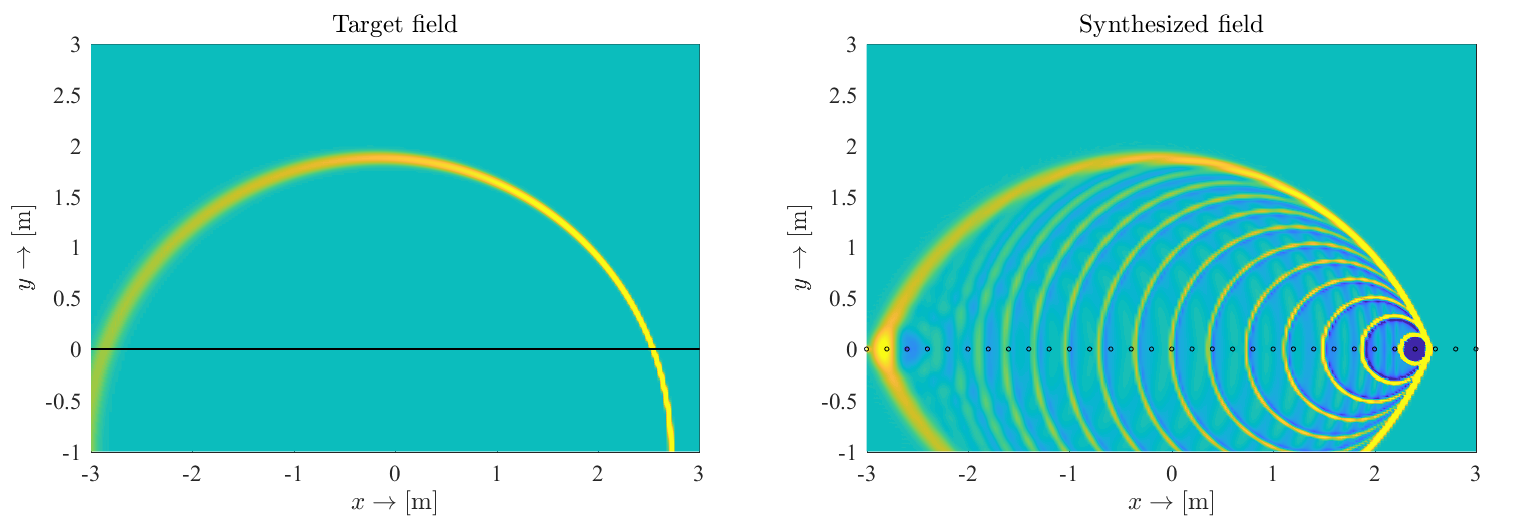
\includegraphics[scale=0.4]{figs/aliasing_artifact.png} \end{figure}\end{center}

\end{frame}

\begin{frame}
\frametitle{Thesis group IV: SDM of moving sources}
\small
Avoiding spatial aliasing
\only<1>{\begin{center}\begin{figure} \includegraphics[scale=0.4]{figs/antialiased_synth_moving_source.png} \end{figure}\end{center}}
%\only<2>{
%\includemedia[
%  width=1\linewidth,
%  height=0.425\linewidth, % 16:9
%  addresource= vids/aliasing.mp4, 
%  transparent,
%  activate=pageopen,
%  passcontext,
%  flashvars={
%  source= vids/aliasing.mp4
%  &autoPlay=true % start playing on activation
%  &loop=true
%  }
%]{}{VPlayer.swf} }
\begin{itemize}
\vspace{-3mm}
\item Anti-aliasing criterion: by time-varying filtering
		\begin{equation*}
		D(\vxo,\omega) = 0, \hspace{5mm} \omega(\vxo,t) \geq \frac{\pi}{\Delta x} \frac{c}{| \hat{k}^P_t(\vxo,t) |}
		\end{equation*}
\vspace{-2mm}
\item Circular SSD: optimal in the aspect of aliasing and referencing the synthesis
\end{itemize}
\end{frame}

\begin{frame}
\frametitle{Thesis group III: Wave Field Synthesis of moving point sources}
Thesis group summary:
	\vspace{3mm}	
	\begin{itemize}
	\item 3D Wave Field Synthesis for moving sources on arbitrary trajectory and excitation signal
	\vspace{3mm}	
	\item 2.5D Wave Field Synthesis for moving sources on arbitrary trajectory and excitation signal, obtained by adapting the stationary phase approximation for time variant field
	\vspace{3mm}	
	\item Closed form 2.5D WFS driving functions for sources under uniform motion ($\leftrightarrow$ arbitrary case: propagation time delay must be expressed apriori)
	\vspace{3mm}	
	\item Frequency-domain 2.5D WFS driving functions for sources under uniform motion, derived directly in the frequency domain
	\end{itemize}
\end{frame}

\begin{frame}
\frametitle{Thesis group IV: Synthesis of moving sources in the wavenumber domain}
Thesis group summary:
	\vspace{3mm}	
	\begin{itemize}
	\item 2.5D SDM driving functions for sources in uniform motion
	\vspace{3mm}	
	\item Proof, for frequency-domain 2.5D WFS and 2.5 SDM driving functions coincide (similarly to the static case)
	\vspace{3mm}	
	\item Analytical treatment of spatial aliasing artifacts regarding frequency distortion artifacts and optimal SSD shape choice
	\vspace{3mm}	
	\item Extension of the novel anti-aliasing strategy for the case of moving sources
	\end{itemize}
\end{frame}

\section{Summary}
\begin{frame}
\frametitle{Summary}
\begin{itemize}
\item Main results
	\vspace{3mm}	
	\begin{itemize}
	\item Unified Wave Field Synthesis framework for arbitrary virtual fields and SSD shapes	\vspace{3mm}	
	\item Spatial form of the explicit approach, proven to coincide with the unified WFS solution 	\vspace{3mm}	
	\item 2.5D WFS and explicit driving function for sources, moving on arbitrary trajectories 	\vspace{3mm}	
	\item Novel anti-aliasing strategy for both static and dynamic virtual fields
	\end{itemize}
\item Outlook
	\begin{itemize}
	\item Discussion of focused virtual sources	\vspace{3mm}	
	\item Efficient implementation of the results
	\end{itemize}
\end{itemize}
\end{frame}

\begin{frame}
\Huge{\centerline{Thank you for the attention!}}
\end{frame}

%----------------------------------------------------------------------------------------

\end{document}